\documentclass[7pt]{article}
\usepackage[left=1in, right=1in, top=1in, bottom=1in]{geometry}
\usepackage[latin1]{inputenc}
\usepackage{amsmath}
\usepackage{amsfonts}
\usepackage{amssymb}
\usepackage{graphicx}
\usepackage{dsfont}
\usepackage{graphicx}
\author{Ben Larson}
\title{Optimization: Homework 4}
\begin{document}
	\maketitle
	\section{Question 1, 5.1}
	Implementing the conjugate gradient method as in Algorithm 5.2. We used it to solve the Hilbert matrix defined as: 
	$$ A_{i,j} = \frac{1}{i+j-1}  \verb|  and   | b = (1,1,....1)^T  \verb |  with   | x_0=0$$ for various dimensions. This algorithm works by trying to minimize the residual in the function: 
	$$ \phi(x) = x^TAx - b^Tx $$
	For each step: 
	$$ stepsize = \alpha_k = \frac{r_k^Tr_k}{p_k^TAp_k} $$
	Then we update the new x with the usual way we have. By a step length above and direction given: 
	$$ p_{k+1} = -r_{k+1} + \beta_{k+1}p_k $$
	This algorithm will converge in n steps. This means that each step/direction is in a conjugate direction. I believe this means that it makes a maximum move in the respective dimension that minimizes the projection of that vector in the subspace of overall function. So each step is a reduction on that dimension.  
\begin{figure}[ht]
	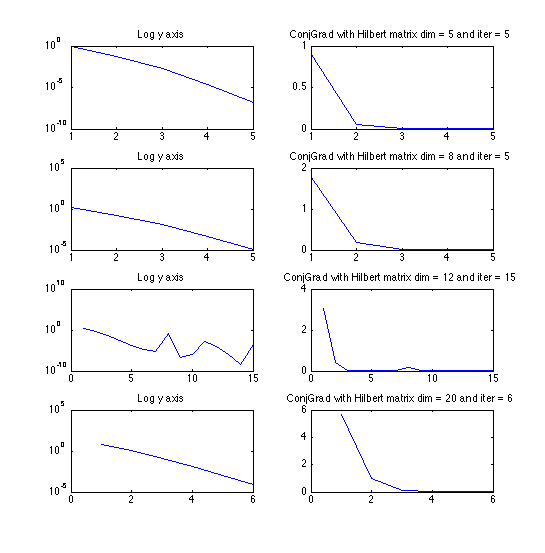
\includegraphics[width=15cm]{untitled}
	\centering
	\caption{Plots of the conjugate gradient minimization on the Hilbert matrix. I tried with dimensions 5,8,12, and 20. Dim = [5, 8] we have the same rate of convergence. Convergence was defined as the residual error less that $10^{-6}$. }
\end{figure}
\section{Question 2, 5.2}
Show that non-zero vectors $p_0,p_1,...p_n$ satisfy: 
$$ p_i^TAp_j=0\verb|  for all  | i\ne j$$ 
where A is symmetric positive definite, then these vectors are linearly independent. \\
We know if the dot product of two vectors, $p_i^Tp_j = 0$ we have orthogonal vectors. If we say that a set of vectors $p_1,p_2...p_n$ can be written linearly independent if $\sum_{i=1}^{n}\alpha_i x_i = 0$ implies that $\alpha_k$=0. This is saying the only way to represent 0 is by setting $\alpha$ =0. In a similar saying, we can say that the only way for any set of vectors to have 0 inner product is if they are orthogonal vectors. $ \sum \alpha_i  p_i^TAp_j = 0$ only if $\alpha_i$=0. 
\section{Question 3, 5.11} 
When applied to a quadratic function, both PR and HS reduce down to FR. 
$$FR = B_{k+1} = \frac{\triangledown f_{k+1}^T \triangledown f_{k+1} }{\triangledown f_k^T\triangledown f_k}$$
$$ PR = \frac{\triangledown f_{k+1}^T(\triangledown f_{k+1}-\triangledown f_k)}{||\triangledown f_k||^2} $$
$$ HS = \frac{\triangledown_{k+1}^T(\triangledown f_{k+1} -\triangledown f_k)}{(\triangledown f_{k+1}-\triangledown f_k)^T p_k} $$
\begin{enumerate}
\item Starting with Polak-Riviere is the easiest to show. We know that for the conjugate gradient methods we get orthogonal vectors with each step. So any vector in $v_{k+1}$ will be orthogonal to $v_k$. This indicates that $v^Tv = 0$. 
$$ PR = \frac{\triangledown f_{k+1}^T(\triangledown f_{k+1}-\triangledown f_k)}{||\triangledown f_k||^2}  = 
 \frac{\triangledown f_{k+1}^T \triangledown f_{k+1} -\triangledown f_k \triangledown f_{k+1}^T )}{\triangledown f_k^T \triangledown f_k} =  \frac{\triangledown f_{k+1}^T \triangledown f_{k+1} -0 }{\triangledown f_k^T \triangledown f_k} $$
And we end up with: 
$$  \frac{\triangledown f_{k+1}^T \triangledown f_{k+1} }{\triangledown f_k^T\triangledown f_k} $$
\item This one I'm not completely sure how to reduce down to the Feltcher Reeves. Starting with: 
$$ HS = \frac{\triangledown_{k+1}^T(\triangledown f_{k+1} -\triangledown f_k)}{(\triangledown f_{k+1}-\triangledown f_k)^T p_k} = \frac{\triangledown f_{k+1}^T\triangledown f_{k+1} -0}{(\triangledown f_{k+1}-\triangledown f_k)^T p_k} = ? ? $$
The consecutive search directions are conjugate with respect to the average hessian on the interval $[x_k,x_{k+1}]$. 
$$G_k = \int \triangledown^2 f(x_k+\tau \alpha_k p_k)d\tau$$
$$ \triangledown f_{k+1} = \triangledown f_k +\alpha_k G_k p_k $$
$$ p_{k+1} = -\triangledown f_{k+1} +\beta_{k+1} p_k $$ 
The condition $p^T_{k+1} G_k p_k = 0$ requires that $\beta_k$ be given by above. Substitute in $\triangledown f_{k+1}$ to the denominator.
$$\frac{\triangledown f_{k+1}^T\triangledown f_{k+1} -0}{(\triangledown f_{k+1}-\triangledown f_k)^T p_k} = \frac{\triangledown f_{k+1}^T\triangledown f_{k+1}}{(\triangledown f_k +\alpha_k G_k p_k-\triangledown f_k)^T p_k} =
\frac{\triangledown f_{k+1}^T\triangledown f_{k+1}}{(\alpha_k G_k p_k)^T p_k}$$
I haven't yet thought of a way to further reduce this. 
\end{enumerate}
	\end{document}